\documentclass[a4paper,11pt]{article}
\usepackage[utf8]{inputenc}		%importing various packages to use
\usepackage{graphicx}
\usepackage{float}
\usepackage{amsmath}
\usepackage{booktabs}

\title{\huge Data Analysis Assignment \\ \hrulefill}

\author{173050043 }
\begin{document}
\maketitle		%making title visible

\section{Introduction}
\label{sec:int}
{\fontfamily{lmr}\fontsize{10}{20}\selectfont		%changing font style,size and formatting
This is the programming assignment of \textbf{\textit{Software Lab Course (CS699)}}. In this assignment our aim is to do data analysis on a xls file which contain the statistic of import and export of India.}
\subsection{Description of Input data}
The input data consist of two files:-
\begin{enumerate}						%making use of bullets
\item India\_Imports\_2011-12\_And\_2012-13.xls
\item India\_Exports\_2011-12\_And\_2012-13.xls
\end{enumerate}

Each of these files contain data about:-
\begin{itemize}						%making use of bullets
\item  Commodity
\item  Country
\item  Unit
\item  Quantity-2011-12
\item  Value-INR-2011-12
\item  Quantity-2012-13
\item  Value-INR-2012-13
\end{itemize}
				%making use of paragraph
\paragraph{Commodity:-} It contain the name of the commodity Imported/Exported by India.
\paragraph{Country:-} It contain the name of the Country with which Import/Export  is done.
\paragraph{Unit:-} It  defines unit in which the quantity is defined.
\paragraph{Quantity:-} It contains the quantity of the Commodity Exported/Imported.
\paragraph{Value:-} It contains the value of the Commodity Exported/Imported.

\section{Objective}				%using bullets in different styles
\label{sec:obj}
Objective of this assignment was to:-
\begin{itemize}
\item[$\Rightarrow$] Getting top 5 import and export destination
\item[$\Rightarrow$] Getting top 5 imort and export commodity
\item[$\Rightarrow$] Preparing single tablelong with trade defict and import-export ratio
\item[$\Rightarrow$] Implementing the use of query function
\item[$\Rightarrow$] Learning how to rename the columns
\item[$\Rightarrow$] Implementing the use of melt function
\item[$\Rightarrow$] Learning how to do intersectiion of table
\end{itemize}



\section{Graphs}					%adding various graphs geerated from figure.py code
\label{sec:gra}
We can conclude following graphs from the input file provided
\subsection{Pie  Chart}
\begin{figure}[H]
\centering
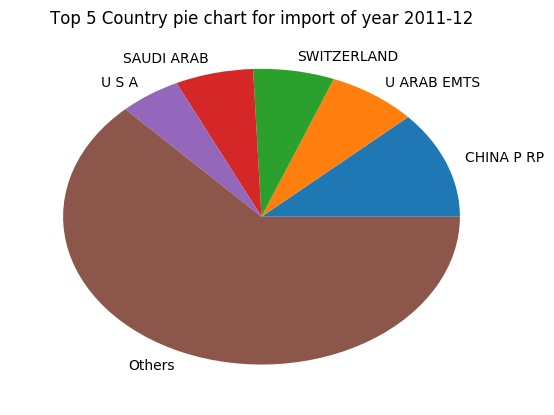
\includegraphics[scale=0.80,width=\textwidth]{image1.jpg}
  \caption{Import Pie Chart}
  \label{fig:pie1}
  
\end{figure}

Figure \ref{fig:pie1} shows Pie chart . It shows the total value imported by top 5 countries and other countries.


\begin{figure}[H]
\centering
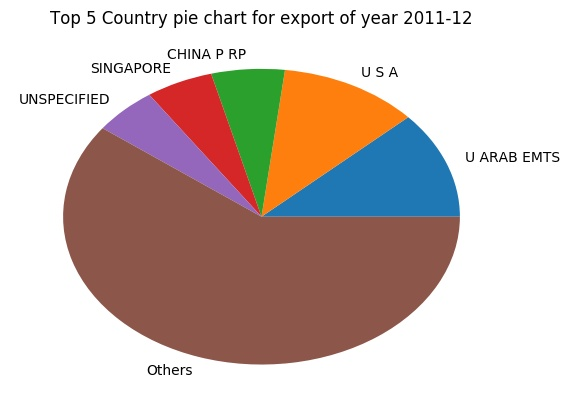
\includegraphics[scale=0.80,width=\textwidth]{image2.jpg}
  \caption{Export Pie Chart}
  \label{fig:pie2}
  
\end{figure}

Figure \ref{fig:pie2} shows Pie chart .It shows the total value exported by top 5 countries and other countries.


\subsection{Bar Graph}
\begin{figure}[H]
\centering
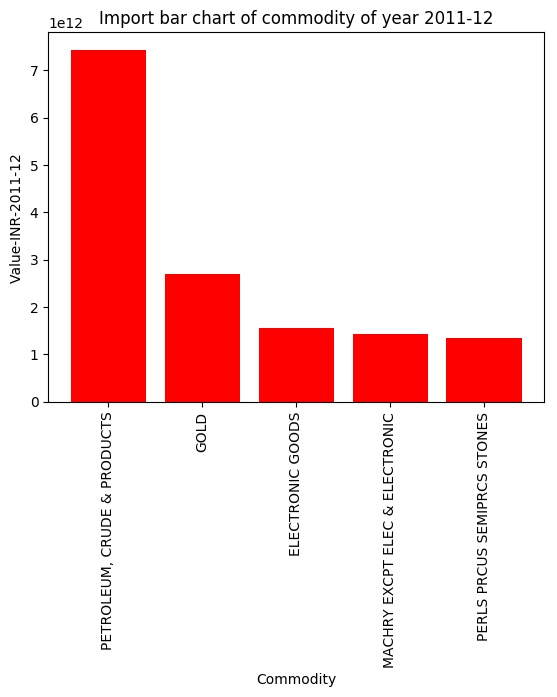
\includegraphics[scale=0.70,width=\textwidth]{image3.jpg}
  \caption{Import Bar Graph}
  \label{fig:bar1}
  
\end{figure}

Figure \ref{fig:bar1} shows a Bar Graph . It compare the import of top 5  commodities with respect to values.


\begin{figure}[H]
\centering
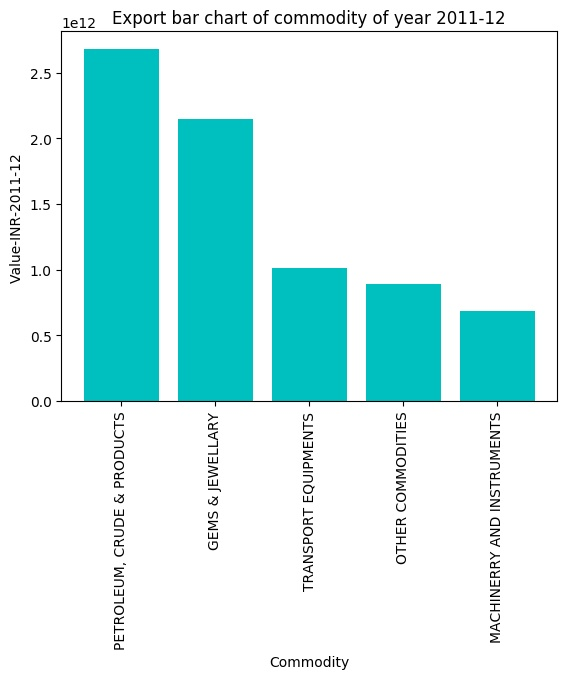
\includegraphics[scale=0.70,width=\textwidth]{image4.jpg}
  \caption{Export Bar Graph}
  \label{fig:bar2}
  
\end{figure}

Figure \ref{fig:bar2} shows Pie chart . It compare the export of top 5  commodities with respect to values.

\subsection{Plot line}
\begin{figure}[H]
\centering
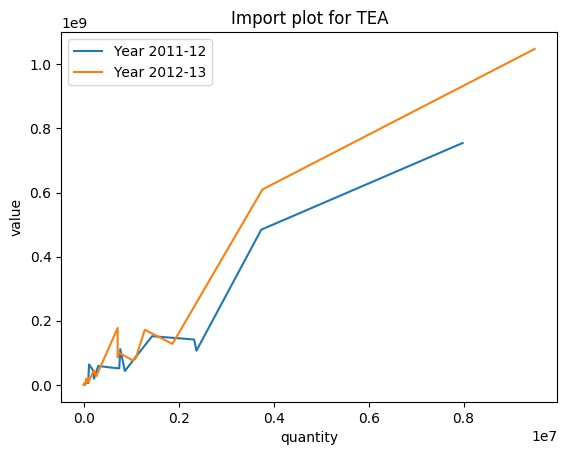
\includegraphics[scale=0.80,width=\textwidth]{image5.jpg}
  \caption{Import Plot Line for Tea}
  \label{fig:plot1}
  
  
  
\end{figure}

Figure \ref{fig:pie1} shows Plot line graph . It shows the quantity vs value plot of import for different years for the commodity TEA.


\begin{figure}[H]
\centering
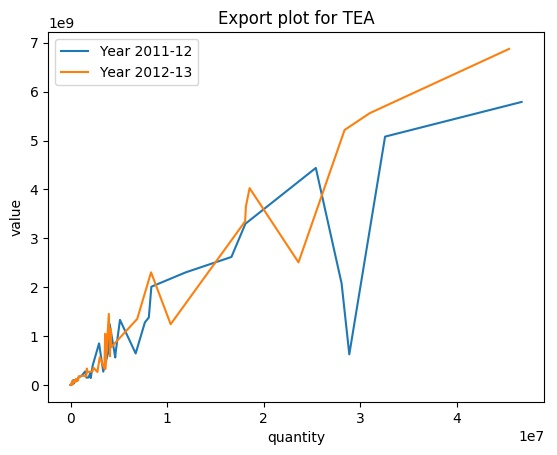
\includegraphics[scale=0.80,width=\textwidth]{image6.jpg}
  \caption{Export Plot Line for Tea}
  \label{fig:plot2}
  
\end{figure}

Figure \ref{fig:plot2} shows Plot line graph. It shows the quantity vs value plot of export for different years for the commodity TEA.


\subsection{Scatter Plot}
\begin{figure}[H]
\centering
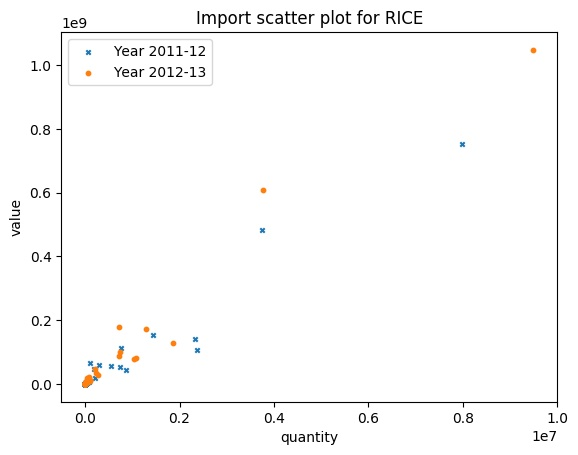
\includegraphics[scale=0.80,width=\textwidth]{image7.jpg}
  \caption{Import Scatter plot for Rice}
  \label{fig:sc1}
  
\end{figure}

Figure \ref{fig:sc1} shows Scatter Plot. It shows the quantity vs value scatter plot of import for different years for the commodity RICE.


\begin{figure}[H]
\centering
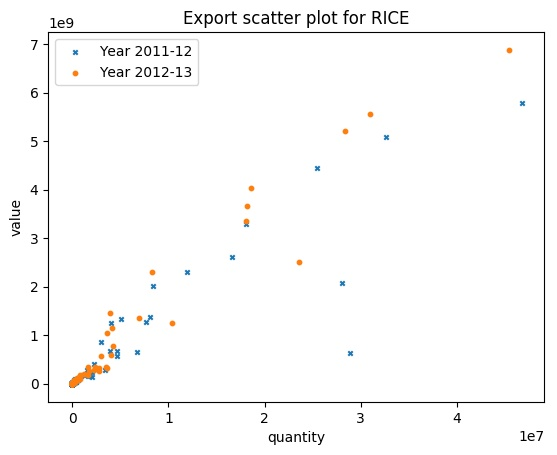
\includegraphics[scale=0.80,width=\textwidth]{image8.jpg}
  \caption{Export Scatter plot for Rice}
  \label{fig:sc2}
  
\end{figure}

Figure \ref{fig:sc2} shows Scatter Plot. It shows the quantity vs value scatter plot of export for different years for the commodity RICE.


\subsection{Histogram}
\begin{figure}[H]
\centering
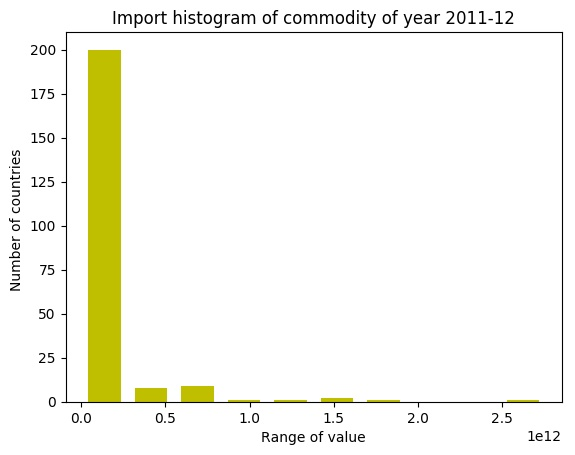
\includegraphics[scale=0.80,width=\textwidth]{image9.jpg}
  \caption{Import Scatter plot for Rice}
  \label{fig:his1}
  
\end{figure}

Figure \ref{fig:his1} shows Histogram. This histogram shows number of countries that import for specific range of values.


\begin{figure}[H]
\centering
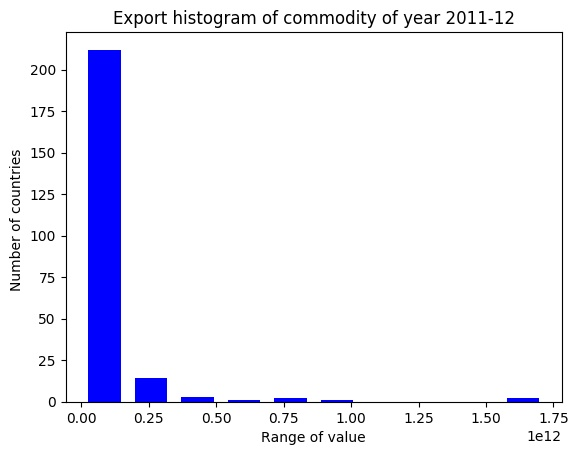
\includegraphics[scale=0.80,width=\textwidth]{image10.jpg}
  \caption{Export Scatter plot for Rice}
  \label{fig:his2}
  
\end{figure}

Figure \ref{fig:his2} shows Histogram. This histogram shows number of countries that export for specific range of values.

\newpage
\section{Mathematical Formula}				%implementing some complex mathematical formula
\label{sec:for}

\subsection{Co relation Formula}
\begin{equation}
cor=
\frac{(\sum_{i=1}^{n}xy)-(\sum_{i=1}^{n}x)(\sum_{i=1}^{n}y)}
{\sqrt{[n\sum_{i=1}^{n}x^2-(\sum_{i=1}^{n}x)^2][n\sum_{i=1}^{n}y^2-(\sum_{i=1}^{n}y)^2]}}
\label{for1}
\end{equation}

\subsection{Combination}

\begin{equation}
\binom nk = \frac{n!}{k!(n-k)!}
\label{for2}
\end{equation}

\subsection{Integration}
\begin{equation}
\int\frac{1}{\sqrt{1-(x)^2}}=sin^{-1}x+c
\label{for3}
\end{equation}

\subsection{Integration By Parts}
\begin{equation}
\int{v\frac{du}{dx}dx}=uv- \int{u\frac{dv}{dx}dx}
\label{for4}
\end{equation}

\section{Table}					%adding table generated from figure.py code
\label{sec:tab}
\begin{table}[H]
\centering
\resizebox{0.60\width}{!}{\begin{tabular}{lrlllrrrr}
\toprule
{} &  index & Commodity &          Country & Unit &  Quantity-2011-12 &  Value-INR-2011-12 &  Quantity-2012-13 &  Value-INR-2012-13 \\
\midrule
0  &    242 &       TEA &            GHANA &  KGS &             24740 &            2376296 &                 0 &                  0 \\
1  &    260 &       TEA &             OMAN &  KGS &            863875 &           43499659 &                 0 &                  0 \\
2  &    269 &       TEA &          SENEGAL &  KGS &             25560 &            3097004 &                 0 &                  0 \\
3  &    232 &       TEA &         BULGARIA &  KGS &             23760 &            2363662 &                 0 &                  0 \\
4  &    238 &       TEA &   CZECH REPUBLIC &  KGS &             20240 &            1065958 &                 0 &                  0 \\
5  &    266 &       TEA &           RUSSIA &  KGS &             13600 &            1982598 &                 0 &                  0 \\
6  &    252 &       TEA &       LUXEMBOURG &  KGS &              2500 &            1812176 &                 0 &                  0 \\
7  &    261 &       TEA &      PAKISTAN IR &  KGS &              1344 &             194681 &                 0 &                  0 \\
8  &    224 &       TEA &          ALBANIA &  KGS &               302 &             139530 &                 0 &                  0 \\
9  &    225 &       TEA &          ANTIGUA &  KGS &             25200 &             954815 &                 0 &                  0 \\
10 &    272 &       TEA &            SPAIN &  KGS &                90 &              26924 &                 0 &                  0 \\
11 &    255 &       TEA &           MEXICO &  KGS &                23 &              46062 &                 0 &                  0 \\
12 &    265 &       TEA &      PUERTO RICO &  KGS &                18 &              18182 &                 0 &                  0 \\
13 &    263 &       TEA &      PHILIPPINES &  KGS &                 2 &               6335 &                 0 &                  0 \\
14 &    246 &       TEA &           ISRAEL &  KGS &                 0 &                  0 &                10 &              20690 \\
15 &    231 &       TEA &          BELGIUM &  KGS &             38515 &            3918695 &                45 &              29181 \\
16 &    258 &       TEA &       NETHERLAND &  KGS &                 0 &                  0 &                68 &              21533 \\
17 &    229 &       TEA &      BAHARAIN IS &  KGS &                 0 &                  0 &                72 &              11124 \\
18 &    243 &       TEA &        HONG KONG &  KGS &              1914 &             718882 &               205 &             100489 \\
19 &    239 &       TEA &       EGYPT A RP &  KGS &                 0 &                  0 &               361 &             222283 \\
20 &    227 &       TEA &        AUSTRALIA &  KGS &              8504 &            3585062 &               390 &            1082737 \\
21 &    230 &       TEA &    BANGLADESH PR &  KGS &                 0 &                  0 &               400 &             186039 \\
22 &    228 &       TEA &          AUSTRIA &  KGS &              8747 &            4382716 &               435 &             279033 \\
23 &    240 &       TEA &           FRANCE &  KGS &               328 &             190118 &               724 &             734413 \\
24 &    233 &       TEA &           CANADA &  KGS &               117 &              54721 &              1190 &            2868549 \\
25 &    270 &       TEA &        SINGAPORE &  KGS &              2745 &             445511 &              2196 &             900897 \\
26 &    259 &       TEA &          NIGERIA &  KGS &                 0 &                  0 &              2287 &             727901 \\
27 &    264 &       TEA &           POLAND &  KGS &                 0 &                  0 &              2380 &             412510 \\
28 &    278 &       TEA &           TURKEY &  KGS &               192 &              29343 &              3378 &             219549 \\
29 &    277 &       TEA &         THAILAND &  KGS &             26554 &            3819801 &              3520 &            1140135 \\
30 &    234 &       TEA &            CHILE &  KGS &                 0 &                  0 &              7703 &            1845903 \\
31 &    235 &       TEA &           TAIWAN &  KGS &             90130 &            5811797 &             10124 &            4577811 \\
32 &    237 &       TEA &          CROATIA &  KGS &                 0 &                  0 &             12000 &            2452140 \\
33 &    254 &       TEA &         MALAYSIA &  KGS &             89549 &            8429539 &             16771 &            3373767 \\
34 &    247 &       TEA &            ITALY &  KGS &             34620 &            6073987 &             22342 &            3601770 \\
35 &    274 &       TEA &           SWEDEN &  KGS &                 0 &                  0 &             24600 &            3635476 \\
36 &    271 &       TEA &     SOUTH AFRICA &  KGS &             46216 &            6606121 &             24837 &            4091225 \\
37 &    256 &       TEA &       MOZAMBIQUE &  KGS &             19500 &            1105418 &             25000 &            3143623 \\
38 &    248 &       TEA &   COTE D' IVOIRE &  KGS &                 0 &                  0 &             25025 &            2159435 \\
39 &    282 &       TEA &          UKRAINE &  KGS &                 0 &                  0 &             27625 &            2790567 \\
40 &    251 &       TEA &         KOREA RP &  KGS &             28072 &            5007017 &             28652 &            4294651 \\
41 &    249 &       TEA &            JAPAN &  KGS &             23829 &            2851395 &             35088 &            5410664 \\
42 &    267 &       TEA &           RWANDA &  KGS &             24500 &            4777177 &             42000 &            8610826 \\
43 &    286 &       TEA &      UNSPECIFIED &  KGS &             13340 &            2366318 &             44000 &            6070593 \\
44 &    241 &       TEA &          GERMANY &  KGS &             37446 &            7313960 &             44137 &           18263116 \\
45 &    280 &       TEA &      U ARAB EMTS &  KGS &            213832 &           19308708 &             56793 &            5923337 \\
46 &    279 &       TEA &           UGANDA &  KGS &             45960 &            4760287 &             70920 &           10377126 \\
47 &    283 &       TEA &            U S A &  KGS &            110243 &           63834911 &             70967 &           16629033 \\
48 &    275 &       TEA &      SWITZERLAND &  KGS &              1459 &             450548 &             88183 &           21607688 \\
49 &    285 &       TEA &         ZIMBABWE &  KGS &                 0 &                  0 &             93240 &            8790146 \\
50 &    268 &       TEA &       SAUDI ARAB &  KGS &             51924 &            6306172 &            107453 &           12032036 \\
51 &    281 &       TEA &              U K &  KGS &            193360 &           46256474 &            212267 &           45418018 \\
52 &    276 &       TEA &     TANZANIA REP &  KGS &             91280 &            7618679 &            235140 &           33778303 \\
53 &    262 &       TEA &      PAPUA N GNA &  KGS &                 0 &                  0 &            262800 &           27538489 \\
54 &    273 &       TEA &    SRI LANKA DSR &  KGS &            303770 &           59203851 &            712866 &          177600862 \\
55 &    253 &       TEA &           MALAWI &  KGS &            554120 &           54451319 &            713314 &           86122998 \\
56 &    236 &       TEA &       CHINA P RP &  KGS &            768909 &          111570421 &            736662 &          100479409 \\
57 &    226 &       TEA &        ARGENTINA &  KGS &           2324180 &          141630070 &           1031578 &           76419725 \\
58 &    284 &       TEA &  VIETNAM SOC REP &  KGS &            746250 &           51607297 &           1088139 &           81292795 \\
59 &    244 &       TEA &        INDONESIA &  KGS &           1437805 &          151993681 &           1285877 &          171952081 \\
60 &    245 &       TEA &             IRAN &  KGS &           2371693 &          106578227 &           1867517 &          127929594 \\
61 &    250 &       TEA &            KENYA &  KGS &           3738669 &          484114505 &           3762870 &          609421144 \\
62 &    257 &       TEA &            NEPAL &  KGS &           7979966 &          754340185 &           9499350 &         1047699721 \\
\bottomrule
\end{tabular}
}
\caption{Tea import table}
\label{tab1}
\end{table}

Table \ref{tab1} represents the deatail of Tea import. It shows all the countriess from which teaa is imported along with quantity and value for the year 2011-12 and 2012-13.

\section{Conclusion}			%Concluding the assignment
\label{sec:con}
From this assignment we learn how to analyse a given set of raw data according to various parameters and extract meaningful information from it.

\section{Summary}				%using reference to all the labels
\label{sec:sum}
This summary contains reference to all table, figure and sections:-
{\fontfamily{pzc}\fontsize{10}{20}\selectfont			%changing font style,size and formatting
\begin{itemize}
\item Section \ref{sec:int} Gives the intoduction of the Assingment
\item Section \ref{sec:obj} Gives the objective of the Assignment
\item Section \ref{sec:gra} Shows all the graphical analysis of the Assignment
	\begin{itemize}
	\item Graph \ref{fig:pie1}	is the pie chart for import
    \item Graph \ref{fig:pie2}	is the pie chart for export
    \item Graph \ref{fig:bar1}	is the bar chart for import
    \item Graph \ref{fig:bar2}	is the bar chart for export
    \item Graph \ref{fig:plot1} is the plot line for tea import
    \item Graph \ref{fig:plot2} is the plot line for tea export
    \item Graph \ref{fig:sc1}	is the scatter plot for rice import
    \item Graph \ref{fig:sc2}	is the scatter plot for rice export
    \item Graph \ref{fig:his1} 	is he histogtam of export (no of country vs range)
    \item Graph \ref{fig:his2} 	is he histogtam of export (no of country vs range)
	\end{itemize}
\item Section \ref{sec:for} Represent some complex mathematical formula
	\begin{itemize}
	\item Formula \ref{for1} is the formula  for co relation
    \item Formula \ref{for2} is the formula  for Combination
    \item Formula \ref{for3} is the formula for Integration
    \item Formula \ref{for4} is the formula for Integration By parts
	\end{itemize}
\item Section \ref{sec:tab} Contains a sub table of the data frame
	\begin{itemize}
	\item Table \ref{tab1} conatins in information about tea import
	\end{itemize}
\item Section \ref{sec:con} contains  the conclusion if the assignment
\item Section \ref{sec:sum} contains summary of the assignment
\end{itemize}

}


\end{document}
